\documentclass[11pt]{article}
\makeatletter\def\input@path{{../}}\makeatother
\usepackage{preamble}
\renewcommand{\chaptername}{Chapter 6: Model selection and diagnostics}
\graphicspath{{figures/}}

\begin{document}

\solutionstitlepage{6}{Model selection and diagnostics}{All numbers and figures are reproduced by \texttt{ch06/code/ch06.R} (base R + MASS + splines).}

\tableofcontents
\clearpage

\section*{Answers at a glance}
\addcontentsline{toc}{section}{Answers at a glance}
\begin{center}
\small
\renewcommand{\arraystretch}{1.25}
\begin{tabular}{>{\bfseries\color{navy}}r p{0.82\linewidth}}\toprule
1  & 5-fold CV clearly prefers $M_2$ (RMSE 22.0 vs 31.3; log score $-500$ vs $-541$).\\
2  & $M_2$ fails PPCs for skewness, maximum and negative values $\Rightarrow$ model $\log(\text{ozone})$ or use a gamma likelihood.\\
3  & DIC/WAIC slightly prefer separate rates ($\approx16$ vs $17$) and are essentially unchanged for $c=1$ vs $10$.\\
4  & Collinear markers: individual effects uncertain, sum precise; posterior spread over overlapping subsets; summarise by region.\\
5  & Logit and probit are indistinguishable (DIC 2525 vs 2527; WAIC 2525 vs 2527).\\
6  & Logistic model under-predicts between-village variation (PPP $\approx0$) $\Rightarrow$ add village random effects.\\
7  & LOO prefers $M_1$ (log score $-23.2$ vs $-24.2$); $\beta_2\approx1$ anyway.\\
8  & $M_2$ passes the PPCs (PPP 0.63); no player is clearly unusual.\\
9  & DIC and WAIC both choose $L=4$.\\
10 & $L=2$ leaves autocorrelated residuals (PPP 0.016) $\Rightarrow$ larger $L$ or a model for differences.\\
11 & $\pi(c)=\frac{n}{(1+nc)^2}$, i.e.\ $c=\frac{U}{n(1-U)}$ with $U\sim\dist{Uniform}(0,1)$.\\
12 & DIC/WAIC pick $J=24$, CV picks $J=18$ (flat for $J=10$--24); residuals autocorrelated.\\
13 & $t$ model passes all four checks; Gaussian fails kurtosis (PPP 0.002).\\
14 & BF: coherent but prior-sensitive; SSVS: many models but needs care with collinearity; CV: assumption-light but costly; DIC/WAIC: cheap but approximate.\\\bottomrule
\end{tabular}
\end{center}
\clearpage

% ================================================================= primer
\section*{A five-minute primer on the tools of this chapter}
\addcontentsline{toc}{section}{Primer: the tools of this chapter}

\begin{recall}
\textbf{1. Cross-validation (CV).} Split the data into $K$ folds; fit the model without fold $k$ and predict fold $k$; repeat for all folds. Score the predictions by mean squared error or by the \emph{log predictive density} $\sum_i\log p(Y_i\mid\mathbf Y_{-\text{fold}(i)})$, estimated by $\log\frac1S\sum_sf(Y_i\mid\theta^{(s)})$. Leave-one-out (LOO) is $K=n$.

\medskip
\textbf{2. DIC.} With deviance $D(\theta)=-2\log f(\mathbf Y\mid\theta)$:
\[
\text{DIC}=\bar D+p_D,\qquad\bar D=\E[D(\theta)\mid\mathbf Y],\qquad p_D=\bar D-D(\hat\theta)\ \ (\hat\theta=\text{posterior mean}).
\]
$p_D$ is the \emph{effective} number of parameters. Smaller DIC is better.

\medskip
\textbf{3. WAIC.} With pointwise draws $\log f(Y_i\mid\theta^{(s)})$:
\[
\text{WAIC}=-2\sum_i\log\overline{f}_i+2p_W,\qquad\overline f_i=\frac1S\sum_sf(Y_i\mid\theta^{(s)}),\qquad p_W=\sum_i\V_s[\log f(Y_i\mid\theta^{(s)})].
\]
It approximates LOO-CV. Smaller is better; a difference of $\gtrsim5$ is usually meaningful.

\medskip
\textbf{4. Posterior predictive checks (PPC).} For each posterior draw, simulate a replicate dataset $\mathbf Y^{\text{rep}}$ of the same size. For a statistic $T$ (mean, max, skewness, autocorrelation, \ldots), compare $T(\mathbf Y)$ with the distribution of $T(\mathbf Y^{\text{rep}})$:
\[
\text{PPP}=\Prob\big(T(\mathbf Y^{\text{rep}})\ge T(\mathbf Y)\mid\mathbf Y\big).
\]
A PPP near 0 or 1 means the model cannot reproduce that feature of the data. Choose statistics that target plausible failures and are \emph{not} directly fitted by the model.
\end{recall}

\clearpage

% ================================================================= Exercise 1
\exercise{6.1 --- Ozone: one predictor or three?}

\begin{problem}{1}
Download the airquality dataset in R. Compare the following two models using 5-fold cross validation:
\begin{align*}
M_1&: \text{ozone}_i\sim\dist{Normal}(\beta_1+\beta_2\,\text{solar.R}_i,\ \sigma^2)\\
M_2&: \text{ozone}_i\sim\dist{Normal}(\beta_1+\beta_2\,\text{solar.R}_i+\beta_3\,\text{temp}_i+\beta_4\,\text{wind}_i,\ \sigma^2).
\end{align*}
Specify and justify the priors you select for both models.
\end{problem}

\begin{restate}
Predict daily ozone in New York either from solar radiation alone, or from solar radiation, temperature and wind; compare the models by how well they predict held-out days.
\end{restate}

\begin{recall}
Bayesian linear regression and its Gibbs sampler (Chapter 4 primer). $K$-fold CV and the log predictive density (primer, point 1).
\end{recall}

\begin{keyidea}
Use the \emph{same} folds for both models, so the comparison is fair, and score both by squared error and by log predictive density (which also rewards honest uncertainty).
\end{keyidea}

\solution
\step{Data.} 111 days with all four variables recorded (days with missing ozone or radiation dropped). Mean ozone 42.1 ppb, SD 33.3.
\step{Priors and justification.} Covariates standardised; $\beta_1,\beta_j\sim\dist N(0,100^2)$ (an SD of 100 ppb per SD of a covariate is far wider than any plausible effect, so the priors are effectively uninformative), $\sigma^2\sim\dist{InvGamma}(0.1,0.1)$ (vague). The same priors are used in both models, so differences come from the data.
\step{5-fold CV} (random folds; for each fold fit by Gibbs on 4/5 of the days and predict the rest):
\begin{center}
\begin{tabular}{lccc}\toprule
 & RMSE (ppb) & MAE (ppb) & log predictive score\\\midrule
$M_1$ & 31.3 & 24.4 & $-540.7$\\
$M_2$ & \textbf{22.0} & \textbf{16.4} & $\mathbf{-500.3}$\\\bottomrule
\end{tabular}
\end{center}
\step{Full-data fits} (coefficients per SD):
\begin{center}
\begin{tabular}{lcc}\toprule
 & $M_1$ mean (95\% CI) & $M_2$ mean (95\% CI)\\\midrule
solar.R & 11.6 (5.8, 17.5) & 5.4 (1.3, 9.7)\\
temp & --- & 15.8 (11.0, 20.5)\\
wind & --- & $-11.8$ $(-16.4,-7.2)$\\
$\sigma$ & 31.5 & 21.3\\\bottomrule
\end{tabular}
\end{center}

\begin{answer}
$M_2$ predicts much better: CV RMSE 22.0 vs.\ 31.3 ppb and log predictive score $-500$ vs.\ $-541$ (a difference of 40 log units is overwhelming). Hot, calm days have much higher ozone; temperature and wind matter more than solar radiation.
\end{answer}

\begin{takeaway}
The log score difference (40) is the CV analogue of a log Bayes factor --- it is huge here. But ``better'' is not ``good'': Exercise 2 shows $M_2$ is still misspecified.
\end{takeaway}

% ================================================================= Exercise 2
\exercise{6.2 --- Posterior predictive checks for the ozone model}

\begin{problem}{2}
Fit model $M_2$ to the airquality data from the previous problem, and use posterior predictive checks to verify that the model fits well. If you find model misspecification, suggest (but do not fit) alternatives.
\end{problem}

\begin{restate}
Simulate fake ozone datasets from the fitted $M_2$ and see whether they look like the real data.
\end{restate}

\begin{recall}
PPC: primer, point 4. Ozone concentrations are positive and right-skewed.
\end{recall}

\begin{keyidea}
Normal linear models are symmetric and can go negative; test statistics that target skewness, extremes and positivity will reveal whether that matters here.
\end{keyidea}

\solution
\step{Replicates.} For each of 10{,}000 posterior draws, $Y_i^{\text{rep}}=\mathbf X_i\bm\beta^{(s)}+\sigma^{(s)}\varepsilon_i$.
\begin{center}
\small
\begin{tabular}{lcccc}\toprule
Statistic $T$ & observed & replicated mean & replicated 95\% interval & PPP\\\midrule
mean & 42.1 & 42.1 & (36.5, 47.7) & 0.50\\
SD & 33.3 & 33.7 & (28.9, 39.1) & 0.54\\
minimum & 1.0 & $-47.5$ & $(-80.6,\ -22.6)$ & \textbf{0.000}\\
maximum & 168 & 122.5 & (101.5, 150.2) & \textbf{0.002}\\
skewness & 1.23 & $-0.11$ & $(-0.51,\ 0.27)$ & \textbf{0.000}\\
share $<0$ & 0 & 0.106 & (0.054, 0.162) & \textbf{1.000}\\\bottomrule
\end{tabular}
\end{center}
\begin{center}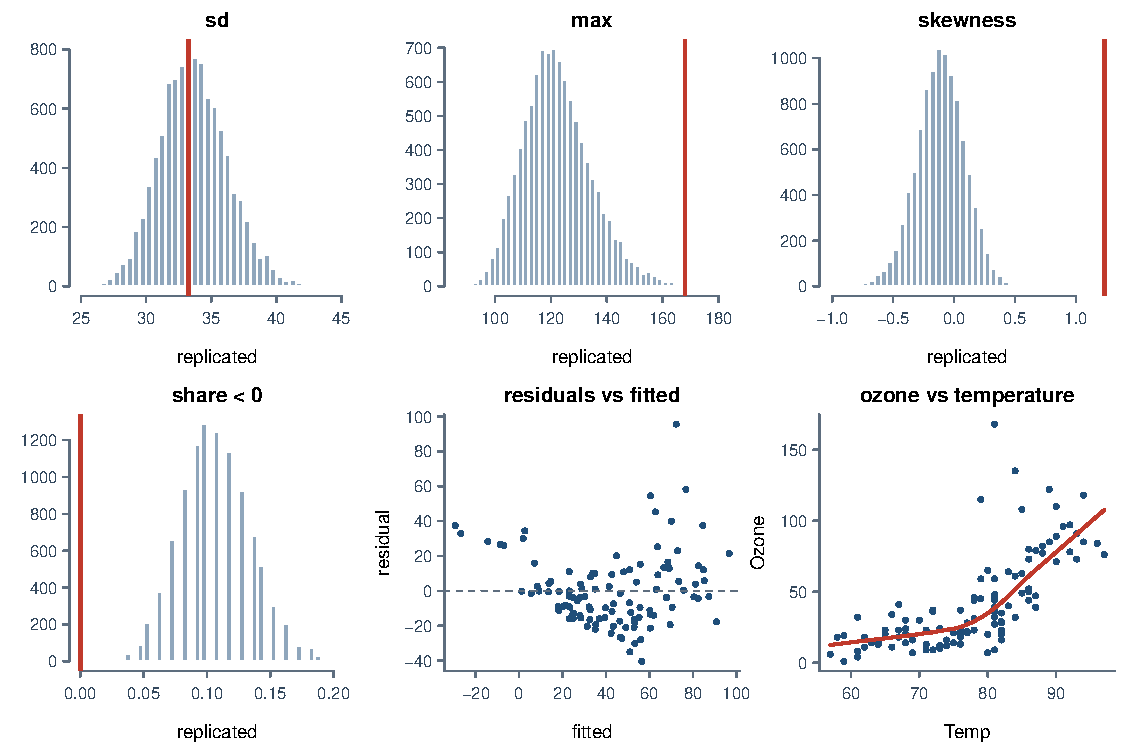
\includegraphics[width=0.98\linewidth]{ex02_ppc.pdf}\end{center}
\step{Diagnosis.} Mean and SD are fine (the model fits them directly), but the replicates are \textbf{symmetric} (skewness $\approx0$ vs.\ 1.23), never reach the observed \textbf{maximum} (168), and about \textbf{11\% of replicated days have negative ozone}. The residual and scatter plots show curvature (ozone rises sharply above $\approx80^\circ$F) and a spread that grows with the fitted value.

\step{Suggested alternatives.}
\begin{itemize}
\item Model $\log(\text{ozone})$ (or a gamma / log-normal likelihood with a log link): positive, right-skewed, variance growing with the mean.
\item Add nonlinear terms: a quadratic or spline in temperature, and a temperature $\times$ wind interaction.
\item Check residual autocorrelation over consecutive days (weather persists).
\end{itemize}

\begin{answer}
$M_2$ reproduces the mean and SD but fails for the minimum, maximum, skewness and positivity (PPP $\approx0$ or 1): it is misspecified. Use a log transform or a gamma likelihood with log link, and allow a nonlinear temperature effect and a temperature--wind interaction.
\end{answer}

\begin{takeaway}
Choose PPC statistics the model does \emph{not} fit by construction; the mean and SD will almost always ``pass''.
\end{takeaway}

% ================================================================= Exercise 3
\exercise{6.3 --- Mr.\ October with DIC and WAIC}

\begin{problem}{3}
Use the ``Mr. October'' data (Section 2.5) $Y_1=563$, $N_1=2820$, $Y_2=10$ and $N_2=27$. Compare the two models:
\begin{align*}
M_1&: Y_1|\lambda_1\sim\dist{Poisson}(N_1\lambda_1)\ \text{and}\ Y_2|\lambda_2\sim\dist{Poisson}(N_2\lambda_2)\\
M_2&: Y_1|\lambda_0\sim\dist{Poisson}(N_1\lambda_0)\ \text{and}\ Y_2|\lambda_0\sim\dist{Poisson}(N_2\lambda_0).
\end{align*}
using DIC and WAIC. Assume the Uniform(0,$c$) prior for all $\lambda_j$, and compare the results for $c=1$ and $c=10$.
\end{problem}

\begin{restate}
Redo Exercise 5.3 (one rate or two?) with DIC and WAIC instead of a Bayes factor.
\end{restate}

\begin{recall}
DIC and WAIC (primer, points 2--3). With a $\dist{Uniform}(0,c)$ prior the posteriors are Gamma distributions truncated at $c$: $\lambda_j\mid\mathbf Y\sim\dist{Gamma}(Y_j+1,N_j)$ on $(0,c)$ under $M_1$, $\lambda_0\mid\mathbf Y\sim\dist{Gamma}(Y_1+Y_2+1,N_1+N_2)$ on $(0,c)$ under $M_2$.
\end{recall}

\begin{keyidea}
DIC and WAIC depend only on the \emph{posterior}, which barely changes with $c$ (the likelihood is concentrated far below $c$). The Bayes factor depends on the \emph{prior density} $1/c$ directly.
\end{keyidea}

\solution
\step{Computation.} Draw $50{,}000$ values from each truncated Gamma posterior (inverse-CDF method), evaluate the two Poisson log-likelihood terms for each draw, then apply the DIC and WAIC formulas (each of the two counts is one ``observation'').
\begin{center}
\begin{tabular}{cc|ccc|ccc}\toprule
$c$ & Model & $\bar D$ & $p_D$ & DIC & lppd & $p_W$ & WAIC\\\midrule
1 & $M_1$ separate & 14.33 & 1.91 & \textbf{16.24} & $-6.86$ & 1.00 & \textbf{15.72}\\
1 & $M_2$ common & 16.44 & 1.01 & 17.45 & $-8.04$ & 0.58 & 17.24\\\midrule
10 & $M_1$ separate & 14.34 & 1.91 & \textbf{16.25} & $-6.86$ & 1.02 & \textbf{15.75}\\
10 & $M_2$ common & 16.44 & 1.00 & 17.44 & $-8.04$ & 0.58 & 17.23\\\bottomrule
\end{tabular}
\end{center}
\why{$p_D\approx2$ and $1$: the effective numbers of parameters match the actual numbers, as expected with weak priors.}

\begin{answer}
Both criteria slightly favour separate rates ($M_1$): DIC 16.2 vs.\ 17.4, WAIC 15.7 vs.\ 17.2 --- differences of about 1.2--1.5, too small to be meaningful. Unlike the Bayes factor in Exercise 5.3 (1.40 vs.\ 0.14), the results are \textbf{essentially identical for $c=1$ and $c=10$}.
\end{answer}

\begin{takeaway}
DIC/WAIC behave like cross-validation (predictive accuracy given the posterior) and are robust to vague priors; Bayes factors measure prior predictive accuracy and are not.
\end{takeaway}

% ================================================================= Exercise 4
\exercise{6.4 --- Variable selection with strongly correlated markers}

\begin{problem}{4}
Consider the regression of the (continuous) CES-D survey score of depression onto $p$ genetic markers. The $p$ covariates for subject $i$, $X_{i1},\dots,X_{ip}$, are aligned along a chromosome giving strong collinearity with the correlation between markers $j$ and $k$ being $\rho^{|j-k|}$ for $\rho=0.99$.
\begin{enumerate}[(a)]
\item Say that $p=3$ and that these generic markers are in fact very important predictors of depression. What do you anticipate the results of Bayesian linear regression with uninformative priors will be?
\item Write a stochastic search variable selection model for these data, and describe how you would summarize the results.
\item Assuming the scenario in (a), what do you anticipate the posterior probability of the $2^p$ models and the $p$ marginal inclusion probabilities will be?
\item Repeat (d) except with $p=1{,}000$. How would you summarize these results?
\end{enumerate}
\end{problem}

\begin{restate}
Three (or 1{,}000) almost identical predictors that genuinely matter: predict what regression and variable selection will report, and how to summarise it.
\end{restate}

\begin{recall}
\begin{itemize}
\item With highly correlated covariates, $\V(\hat{\bm\beta})=\sigma^2(\mathbf X^\top\mathbf X)^{-1}$ is huge for individual coefficients but small for their \emph{sum} (the direction the data identify).
\item SSVS: primer of Chapter 5, point 6.
\end{itemize}
\end{recall}

\begin{keyidea}
The data can tell that \emph{this region} matters, but not \emph{which} of the nearly identical markers carries the signal. To make the predictions concrete we simulated $n=1{,}000$ subjects with $\rho=0.99$ and all three true effects equal to 0.3 (noise SD 1).
\end{keyidea}

\solution
\step{(a) Uninformative priors.} Expect wide, strongly negatively correlated posteriors for $\beta_1,\beta_2,\beta_3$, with individual intervals that may include 0 or even have the wrong sign, while the \emph{sum} $\beta_1+\beta_2+\beta_3$ is precisely estimated. The simulation confirms this:
\begin{center}
\begin{tabular}{lccc}\toprule
 & estimate & SE & truth\\\midrule
$\beta_1$ & 0.39 & 0.22 & 0.3\\
$\beta_2$ & 0.60 & 0.31 & 0.3\\
$\beta_3$ & $-0.05$ & 0.23 & 0.3\\
$\beta_1+\beta_2+\beta_3$ & \textbf{0.94} & \textbf{0.03} & 0.9\\\bottomrule
\end{tabular}
\end{center}
Not one marker is ``significant'' on its own, yet together they are overwhelmingly important.

\step{(b) SSVS model.}
$Y_i=\beta_0+\sum_{j=1}^p\gamma_j\beta_jX_{ij}+\varepsilon_i$, $\gamma_j\iid\dist{Bernoulli}(q)$, $\beta_j\mid\sigma^2\sim\dist N(0,W\sigma^2)$, $\pi(\beta_0)\propto1$, $\pi(\sigma^2)\propto1/\sigma^2$ (with $q\sim\dist{Beta}$ when $p$ is large). Summaries: posterior model probabilities, marginal inclusion probabilities $\Prob(\gamma_j=1\mid\mathbf Y)$, and --- crucially with collinearity --- the probability that \emph{at least one} marker in a correlated block is included.

\step{(c) Model probabilities for $p=3$} (exact, $W=1$):
\begin{center}
\begin{tabular}{lc|lc}\toprule
Model & Probability & Model & Probability\\\midrule
none & 0.000 & $X_3$ & 0.000\\
$X_1$ & 0.066 & $X_1+X_3$ & 0.048\\
$X_2$ & 0.324 & $X_2+X_3$ & 0.071\\
$X_1+X_2$ & \textbf{0.403} & $X_1+X_2+X_3$ & 0.089\\\bottomrule
\end{tabular}
\end{center}
Inclusion probabilities: $X_1$ 0.61, $X_2$ 0.89, $X_3$ 0.21. The null model has probability 0, so ``some marker matters'' has probability 1 --- but the mass is spread over overlapping subsets, and a truly important marker ($X_3$) gets a low inclusion probability.

\step{(d) $p=1{,}000$.} Expect the same, magnified: the posterior wanders among thousands of near-equivalent models; no single model has appreciable probability; inclusion probabilities are diluted across each correlated block (each marker in a block might get 0.05--0.3 even if the block certainly matters), and results can be sensitive to the MCMC run. Summaries should therefore be at the \textbf{region} level:
\begin{itemize}
\item sum the inclusion probabilities over windows of adjacent markers (expected number of active markers per region) and plot along the chromosome;
\item report \emph{credible sets}: the smallest set of markers that contains an active one with 95\% probability (as in genetic fine-mapping);
\item report the posterior distribution of the total genetic contribution (e.g.\ variance explained), which is well identified.
\end{itemize}

\begin{answer}
(a) Individual coefficients wide and negatively correlated (possibly wrong signs), their sum precise. (b) Spike-and-slab SSVS with block-level summaries. (c) Null model probability $\approx0$, but probability spread over several overlapping subsets; marginal inclusion probabilities moderate and uneven (0.61, 0.89, 0.21 in our simulation). (d) Even more dilution; summarise by regions/credible sets rather than individual markers.
\end{answer}

\begin{takeaway}
Low inclusion probabilities do \emph{not} mean ``no effect'' when predictors are collinear --- always look at blocks.
\end{takeaway}

% ================================================================= Exercise 5
\exercise{6.5 --- Logit or probit for the Gambia data?}

\begin{problem}{5}
Use DIC and WAIC to compare logistic and probit links for the gambia data in the R package geoR using the five covariates in Listing 6.2 and no random effects.
\end{problem}

\begin{restate}
Fit the malaria regression with a logistic and a probit link and compare the fits with DIC and WAIC.
\end{restate}

\begin{recall}
Logit link: $\Prob(Y=1)=\frac{e^\eta}{1+e^\eta}$; probit link: $\Prob(Y=1)=\Phi(\eta)$. Both are S-shaped; the logistic curve has slightly heavier tails. Coefficients are related roughly by $\beta_{\text{logit}}\approx1.6\,\beta_{\text{probit}}$.
\end{recall}

\begin{keyidea}
Same covariates (age, bed-net use, treated net, greenness, health centre), same priors ($\beta_j\sim\dist N(0,100)$ as in the book), only the link differs.
\end{keyidea}

\solution
\step{Fit.} Block Metropolis for each link (20{,}000 kept draws, acceptance 27--28\%); pointwise log-likelihoods $Y_i\log p_i+(1-Y_i)\log(1-p_i)$ for every draw.
\begin{center}
\begin{tabular}{lcccccc}\toprule
Link & $\bar D$ & $p_D$ & DIC & lppd & $p_W$ & WAIC\\\midrule
logit & 2519.4 & 5.8 & 2525.2 & $-1256.8$ & 5.9 & 2525.3\\
probit & 2521.0 & 6.1 & 2527.1 & $-1257.4$ & 6.2 & 2527.2\\\bottomrule
\end{tabular}
\end{center}
\why{$p_D\approx p_W\approx6$ = the number of coefficients: the priors are weak.}
\begin{center}
\begin{tabular}{lccc}\toprule
 & logit & probit & ratio\\\midrule
age & 0.274 & 0.167 & 1.64\\
netuse & $-0.564$ & $-0.349$ & 1.62\\
treated & $-0.289$ & $-0.159$ & 1.81\\
green & 0.295 & 0.172 & 1.72\\
phc & $-0.210$ & $-0.134$ & 1.57\\\bottomrule
\end{tabular}
\end{center}

\begin{answer}
DIC 2525.2 (logit) vs.\ 2527.1 (probit); WAIC 2525.3 vs.\ 2527.2. The difference ($\approx2$) is negligible: the two links fit equally well, and their coefficients differ only by the usual factor $\approx1.6$. Choose logit for its odds-ratio interpretation.
\end{answer}

\begin{takeaway}
With probabilities mostly between 0.1 and 0.7, logit and probit curves are almost identical; link choice matters only for extreme probabilities.
\end{takeaway}

% ================================================================= Exercise 6
\exercise{6.6 --- Posterior predictive checks for the Gambia logistic model}

\begin{problem}{6}
Fit logistic regression model to the gambia data in the previous question and use posterior predictive checks to verify the model fits well. If you find model misspecification, suggest (but do not fit) alternatives.
\end{problem}

\begin{restate}
Check whether the logistic model without village effects reproduces key features of the malaria data.
\end{restate}

\begin{recall}
PPC: primer, point 4. Children live in 65 villages; a model without village effects assumes that, given the covariates, villages differ only by chance.
\end{recall}

\begin{keyidea}
Overall prevalence is fitted by construction. The informative statistics are about \emph{between-village} variation, which the model was not told about.
\end{keyidea}

\solution
\step{Replicates.} 4{,}000 posterior draws; for each, simulate $Y_i^{\text{rep}}\sim\dist{Bernoulli}(p_i^{(s)})$ for all 2{,}035 children.
\begin{center}
\small
\begin{tabular}{lcccc}\toprule
Statistic & observed & replicated mean & 95\% interval & PPP\\\midrule
overall prevalence & 0.357 & 0.358 & (0.329, 0.385) & 0.52\\
SD of village prevalence & 0.226 & 0.137 & (0.113, 0.161) & \textbf{0.000}\\
max village prevalence & 0.933 & 0.723 & (0.600, 0.875) & \textbf{0.007}\\
villages with 0 positives & 2 & 0.02 & (0, 0) & \textbf{0.000}\\\bottomrule
\end{tabular}
\end{center}
\begin{center}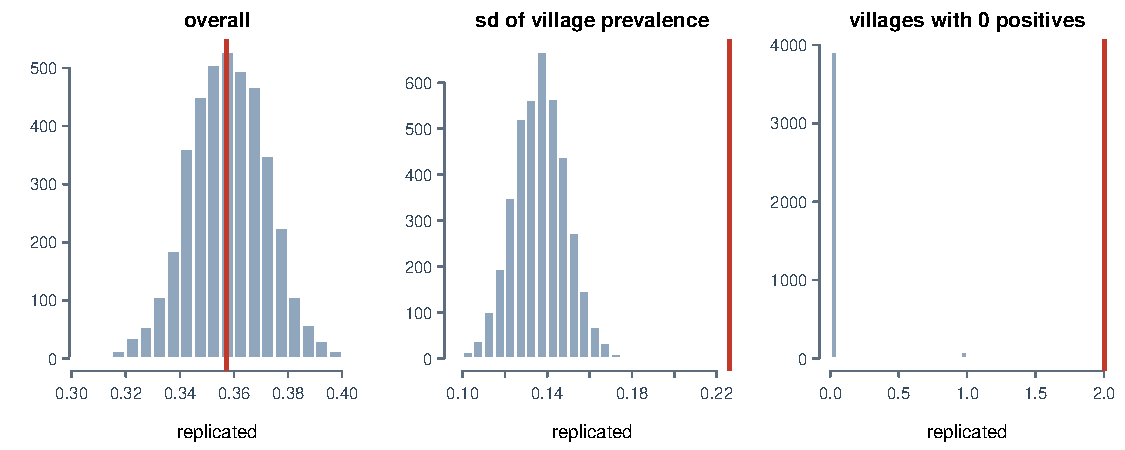
\includegraphics[width=0.98\linewidth]{ex06_ppc.pdf}\end{center}
By age group, the older groups are reproduced, but the youngest children (under 1.5 years) have lower prevalence than the model predicts (0.19 vs.\ a replicated 95\% interval of 0.21--0.32): the linear age effect is too simple.

\step{Diagnosis.} The real villages are far more different from each other than the model allows: the SD of village prevalence is 0.23 vs.\ 0.14 replicated, one village has 93\% positives, and two villages have none --- something the model essentially never produces.

\step{Suggested alternatives.}
\begin{itemize}
\item Village random effects (Exercise 4.8, which estimated $\tau\approx0.8$).
\item Spatially correlated village effects (nearby villages share mosquito habitat), e.g.\ a Gaussian process in the coordinates.
\item A nonlinear age effect (e.g.\ a spline in age), since the youngest children are over-predicted.
\end{itemize}

\begin{answer}
The model matches overall prevalence but over-predicts malaria in the youngest children and badly under-predicts between-village variation (PPP $\approx0$ for the SD of village prevalence and the number of malaria-free villages). Add village (ideally spatially correlated) random effects and a nonlinear age effect.
\end{answer}

\begin{takeaway}
Grouping structure that is ignored by the model shows up as extra variation between groups --- an easy, targeted PPC.
\end{takeaway}

% ================================================================= Exercise 7
\exercise{6.7 --- Leave-one-out comparison of two clutch models}

\begin{problem}{7}
For the NBA free throw data in Section 1.6, assume that for player $i$, $Y_i|p_i\sim\dist{Binomial}(n_i,p_i)$ where $Y_i$ is the number of clutch makes, $n_i$ is the number of clutch attempts, and $p_i$ is the clutch make probability. Use leave-one-out cross validation to compare the models:
\begin{align*}
M_1&: \mathrm{logit}(p_i)=\beta_1+\mathrm{logit}(q_i)\\
M_2&: \mathrm{logit}(p_i)=\beta_1+\beta_2\,\mathrm{logit}(q_i),
\end{align*}
where $q_i$ is the overall free throw percentage.
\end{problem}

\begin{restate}
Is clutch shooting a constant shift of each player's overall percentage on the logit scale ($M_1$), or does the shift depend on how good the player is ($M_2$)? Compare by predicting each player from the other nine.
\end{restate}

\begin{recall}
LOO log score: $\sum_{i=1}^{10}\log p(Y_i\mid\mathbf Y_{-i})$, with $p(Y_i\mid\mathbf Y_{-i})\approx\frac1S\sum_s\dist{Binomial}(Y_i;n_i,p_i^{(s)})$ using draws from the posterior fitted \emph{without} player $i$.
\end{recall}

\begin{keyidea}
$M_1$ is $M_2$ with $\beta_2$ fixed at 1 (a ``logit offset''). With only 10 players the extra parameter has to earn its keep.
\end{keyidea}

\solution
\step{Fits.} Priors $\beta_j\sim\dist N(0,10^2)$; block Metropolis with GLM-based proposals; 10{,}000 kept draws per fit. For LOO, each model is refitted 10 times (once without each player).
\begin{center}
\small
\begin{tabular}{lcc|lcc}\toprule
Player & $M_1$ & $M_2$ & Player & $M_1$ & $M_2$\\\midrule
Westbrook & $-2.45$ & $-2.49$ & Curry & $-1.55$ & $-1.61$\\
Harden & $-3.95$ & $-4.00$ & Antetokounmpo & $-2.39$ & $-2.49$\\
Leonard & $-2.00$ & $-2.07$ & Wall & $-2.63$ & $-2.62$\\
James & $-2.37$ & $-2.84$ & Davis & $-2.32$ & $-2.34$\\
Thomas & $-2.02$ & $-2.26$ & Durant & $-1.51$ & $-1.52$\\\midrule
\multicolumn{6}{c}{Total LOO log score: $M_1$ $\mathbf{-23.18}$, \ $M_2$ $-24.23$ \ (difference $-1.05$, SE 0.46)}\\\bottomrule
\end{tabular}
\end{center}
\step{Full-data posteriors.} $M_1$: $\beta_1=-0.18$ $(-0.39,\ 0.04)$. $M_2$: $\beta_1=-0.13$ $(-0.92,\ 0.66)$, $\beta_2=0.97$ $(0.49,\ 1.47)$.
\why{$M_2$ loses mostly on LeBron James and Isaiah Thomas, the players with the lowest and highest overall rates: when one of them is left out, the slope $\beta_2$ is poorly determined and predictions for extreme players become unstable.}

\begin{answer}
LOO-CV prefers the simpler $M_1$ (log score $-23.2$ vs.\ $-24.2$). Consistently, $M_2$'s slope is $\beta_2\approx0.97$, very close to the value 1 that $M_1$ assumes. Clutch shooting is well described as a common shift of about $-0.18$ on the logit scale (about 2 percentage points lower in the clutch).
\end{answer}

\begin{takeaway}
When the extra parameter's posterior sits at the value the simpler model fixes, CV will (rightly) prefer the simpler model.
\end{takeaway}

% ================================================================= Exercise 8
\exercise{6.8 --- Posterior predictive checks for the clutch model}

\begin{problem}{8}
Fit model $M_2$ to the NBA data in the previous question, and use posterior predictive checks to verify the model fits well. If you find model misspecification, suggest (but do not fit) alternatives.
\end{problem}

\begin{restate}
Can model $M_2$ reproduce each player's clutch makes and the overall spread around the fitted rates?
\end{restate}

\begin{recall}
\textbf{Chi-square discrepancy} $T(\mathbf Y,\theta)=\sum_i\frac{(Y_i-n_ip_i)^2}{n_ip_i(1-p_i)}$: compares observed and replicated spread around the fitted probabilities (detects over-dispersion). Its PPP is $\Prob\{T(\mathbf Y^{\text{rep}},\theta)\ge T(\mathbf Y,\theta)\}$.
\end{recall}

\begin{keyidea}
Check both a global statistic (over-dispersion) and each player individually (is any player's count unusual under the model?).
\end{keyidea}

\solution
\step{Global check.} Mean observed discrepancy 8.1 (about what one expects for 10 binomial counts); $\text{PPP}=0.63$: no sign of over-dispersion.
\step{Player-level checks.}
\begin{center}
\small
\begin{tabular}{lccc}\toprule
Player & observed makes & 95\% predictive interval & $\Prob(Y^{\text{rep}}\le Y)$\\\midrule
Westbrook & 64 & (54, 68) & 0.80\\
Harden & 72 & (70, 86) & \textbf{0.09}\\
Leonard & 55 & (48, 59) & 0.67\\
James & 27 & (18, 32) & 0.76\\
Thomas & 75 & (67, 80) & 0.67\\
Curry & 24 & (19, 26) & 0.83\\
Antetokounmpo & 28 & (24, 36) & 0.28\\
Wall & 66 & (55, 71) & 0.78\\
Davis & 40 & (35, 48) & 0.35\\
Durant & 13 & (10, 16) & 0.43\\\bottomrule
\end{tabular}
\end{center}
\begin{center}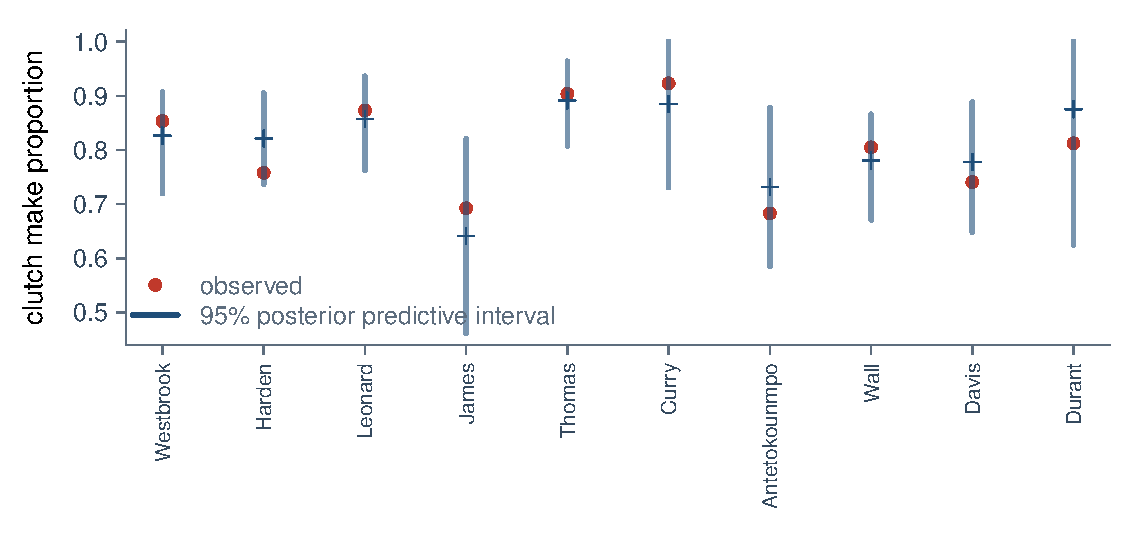
\includegraphics[width=0.85\linewidth]{ex08_ppc.pdf}\end{center}
Every observed count lies inside its 95\% predictive interval. Harden is at the low edge ($\Prob(Y^{\text{rep}}\le72)=0.09$), consistent with Chapter 1's finding, but with 10 players one value near 0.1 is expected by chance.

\step{If misfit had appeared.} Add a player-level random effect, $\mathrm{logit}(p_i)=\beta_1+\beta_2\mathrm{logit}(q_i)+u_i$ with $u_i\sim\dist N(0,\tau^2)$ (equivalently a beta-binomial likelihood), to allow genuine individual clutch effects.

\begin{answer}
$M_2$ fits well: chi-square PPP $=0.63$ and every player's makes fall within their 95\% predictive interval. Harden is the most unusual (PPP 0.09) but not alarming. If needed, a player random effect (beta-binomial) would capture individual clutch effects.
\end{answer}

\begin{takeaway}
Combine a global discrepancy with unit-level checks: global statistics can hide one badly fitted unit.
\end{takeaway}

% ================================================================= Exercise 9
\exercise{6.9 --- Choosing the lag of an autoregression for web traffic}

\begin{problem}{9}
Download the WWWusage dataset in R. Using data from times $t=5,\dots,100$ as outcomes (earlier times may be used as covariates), fit the autoregressive model
\[
Y_t|Y_{t-1},\dots,Y_1\sim\dist{Normal}(\beta_0+\beta_1Y_{t-1}+\dots+\beta_LY_{t-L},\ \sigma^2)
\]
where $Y_t$ is the WWW usage at time $t$. Compare the models with $L=1,2,3,4$, and select the best time lag $L$.
\end{problem}

\begin{restate}
The number of users connected to a server each minute: predict it from the previous 1--4 minutes and pick how many lags to use.
\end{restate}

\begin{recall}
Conditional on the first values, an AR($L$) model is a linear regression of $Y_t$ on $(Y_{t-1},\dots,Y_{t-L})$, so the Gibbs sampler of Chapter 4 applies. Using the same outcomes ($t=5,\dots,100$) for every $L$ makes the criteria comparable.
\end{recall}

\begin{keyidea}
Compare DIC and WAIC across $L$ (same 96 outcomes, vague priors $\dist N(0,100^2)$, $\sigma^2\sim\dist{InvGamma}(0.1,0.1)$).
\end{keyidea}

\solution
\begin{center}
\begin{tabular}{ccccccc}\toprule
$L$ & $\bar D$ & $p_D$ & DIC & lppd & $p_W$ & WAIC\\\midrule
1 & 609.8 & 3.0 & 612.8 & $-303.6$ & 2.6 & 612.4\\
2 & 508.1 & 4.0 & 512.1 & $-252.3$ & 3.7 & 512.0\\
3 & 502.0 & 5.0 & 507.0 & $-248.7$ & 4.9 & 507.1\\
4 & 487.0 & 5.9 & \textbf{492.9} & $-240.9$ & 5.6 & \textbf{493.0}\\\bottomrule
\end{tabular}
\end{center}
Posterior means for $L=4$: $\beta_1=2.12$, $\beta_2=-1.81$, $\beta_3=1.06$, $\beta_4=-0.40$ (all 95\% intervals exclude 0), $\sigma=3.06$.
\why{Each extra lag lowers DIC/WAIC by more than 5, and the fourth lag still by 14: the series has smooth, wave-like dynamics that need several lags to describe.}

\begin{answer}
DIC and WAIC agree: $L=4$ is best (DIC 492.9, WAIC 493.0), clearly better than $L=3$ ($\approx507$). Select $L=4$ (within the lags considered).
\end{answer}

\begin{takeaway}
$\beta_1\approx1$ for $L=1$ and $\sum_l\beta_l\approx0.98$ for $L=4$: the series is close to non-stationary, suggesting a model for the \emph{differences} $Y_t-Y_{t-1}$ (Exercise 10).
\end{takeaway}

% ================================================================= Exercise 10
\exercise{6.10 --- Checking the AR(2) model for web traffic}

\begin{problem}{10}
Using the WWWusage dataset in the previous problem, fit the model with $L=2$ and use posterior predictive checks to verify that the model fits well. If you find model misspecification, suggest (but do not fit) alternatives.
\end{problem}

\begin{restate}
Do the AR(2) model's residuals behave like independent noise?
\end{restate}

\begin{recall}
If the model is right, the errors $\varepsilon_t=Y_t-\mu_t$ are independent $\dist N(0,\sigma^2)$, so their autocorrelation should be near 0. Replicated errors $\varepsilon_t^{\text{rep}}=Y_t^{\text{rep}}-\mu_t$ show what ``near 0'' means for 96 points.
\end{recall}

\begin{keyidea}
For time series, the best PPC statistics are residual autocorrelations at lags 1 and 2, plus kurtosis and the largest absolute residual.
\end{keyidea}

\solution
\step{Statistics} (averaged over posterior draws; PPP $=\Prob(T^{\text{rep}}\ge T^{\text{obs}})$):
\begin{center}
\begin{tabular}{lcccc}\toprule
 & lag-1 ACF & lag-2 ACF & kurtosis & max $|\varepsilon|$\\\midrule
observed & 0.225 & $-0.314$ & $-0.32$ & 8.5\\
replicated & $-0.010$ & $-0.009$ & $-0.12$ & 9.3\\
PPP & \textbf{0.016} & \textbf{0.993} & 0.63 & 0.67\\\bottomrule
\end{tabular}
\end{center}
\begin{center}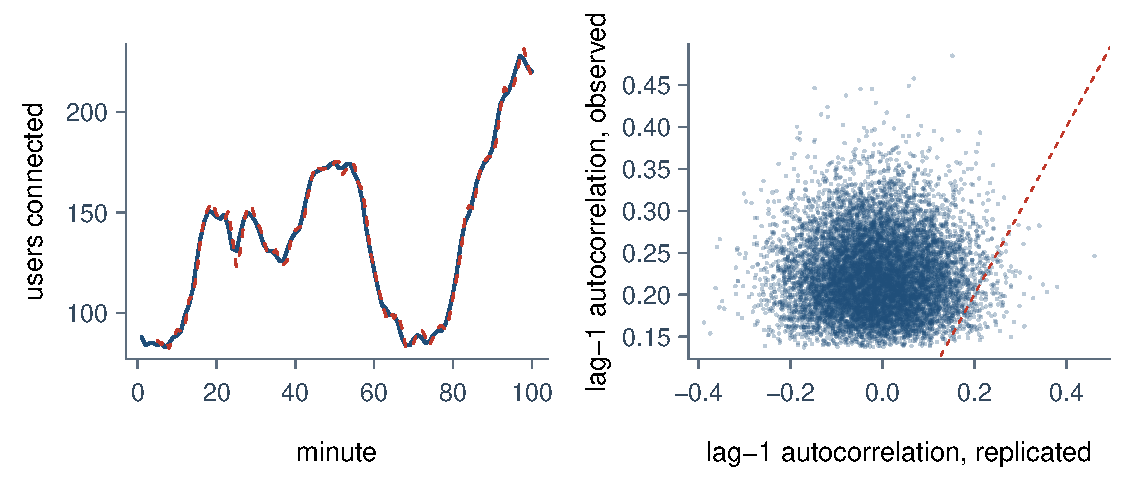
\includegraphics[width=0.98\linewidth]{ex10_ppc.pdf}\end{center}
The residuals are clearly autocorrelated (positive at lag 1, negative at lag 2), which independent noise essentially never produces; tails/extremes are fine.

\step{Suggested alternatives.}
\begin{itemize}
\item More lags ($L=3,4$ --- as Exercise 9 already found).
\item Model the differences: an AR model for $\Delta Y_t=Y_t-Y_{t-1}$ (an ARIMA$(p,1,0)$), since the series behaves like an integrated process (the differences have lag-1 autocorrelation 0.79).
\item Possibly time-varying variance (the series has calm and volatile stretches).
\end{itemize}

\begin{answer}
The AR(2) model fails the residual-autocorrelation checks (lag-1 PPP 0.016, lag-2 PPP 0.993), so it is misspecified; kurtosis and extremes are fine. Use more lags or, better, an AR model for the first differences (ARIMA).
\end{answer}

\begin{takeaway}
For time series, ``independent errors'' is the assumption most worth checking.
\end{takeaway}

% ================================================================= Exercise 11
\exercise{6.11 --- A prior that makes $p_D$ uniform}

\begin{problem}{11}
For the one-way random effects model in (6.12), explain how you would select a prior for $c$ so the $p_D$ has roughly a uniform prior on $p_D$.
\end{problem}

\begin{restate}
In the random-effects model, the effective number of parameters $p_D$ depends on the prior variance ratio $c$. Choose a prior for $c$ that makes every model size between 0 and $p$ equally likely.
\end{restate}

\begin{recall}
Model (6.12): $Y_{ij}\mid\mu_j\sim\dist N(\mu_j,\sigma^2)$, $\mu_j\sim\dist N(0,c\sigma^2)$, $n$ replicates in each of $p$ groups. The book shows $p_D=p\,\frac{c}{c+1/n}$.
\textbf{Change of variables}: if $U=g(c)$ and we want $U\sim\dist{Uniform}(0,1)$, then $c=g^{-1}(U)$ and $\pi(c)=|g'(c)|$.
\end{recall}

\begin{keyidea}
Make $U=p_D/p=\frac{c}{c+1/n}=\frac{nc}{1+nc}$ uniform on $(0,1)$ and solve for $c$.
\end{keyidea}

\solution
\step{Step 1 --- invert.} $U=\frac{nc}{1+nc}\iff U+Unc=nc\iff c=\frac{U}{n(1-U)}$.
\step{Step 2 --- the implied density.} $\frac{\dd U}{\dd c}=\frac{n(1+nc)-nc\cdot n}{(1+nc)^2}=\frac{n}{(1+nc)^2}$, so
\[
\pi(c)=\frac{n}{(1+nc)^2},\qquad c>0.
\]
This is proper ($\int_0^\infty\frac{n}{(1+nc)^2}\dd c=1$), with median $1/n$ and a heavy right tail. Equivalently $nc$ has the ``beta-prime$(1,1)$'' (log-logistic) distribution.
\step{Step 3 --- in practice.} Either use this density directly, or put a $\dist{Uniform}(0,1)$ prior on $U$ (the ``shrinkage fraction'') and define $c=U/\{n(1-U)\}$ in the model code. If group sizes differ, the same idea applies with $n$ replaced by a typical group size (making $p_D$ approximately uniform).

\begin{sanity}
Simulation with $n=5$, $p=10$: $10^5$ draws of $c$ give $p_D$ with mean 4.997 (theory 5) and a KS distance of 0.002 from $\dist{Uniform}(0,10)$; the median of $c$ is $0.199\approx1/5$. \checkmark
\end{sanity}

\begin{answer}
Set $c=\dfrac{U}{n(1-U)}$ with $U\sim\dist{Uniform}(0,1)$, i.e.\ $\pi(c)=\dfrac{n}{(1+nc)^2}$; then $p_D/p=\frac{c}{c+1/n}=U$ is uniform, so $p_D\sim\dist{Uniform}(0,p)$.
\end{answer}

\begin{takeaway}
Putting priors on interpretable quantities (``how much shrinkage'', ``effective model size'') is a principled way to choose priors for variance parameters.
\end{takeaway}

% ================================================================= Exercise 12
\exercise{6.12 --- How many spline basis functions for the temperature curve?}

\begin{problem}{12}
The global mean temperature anomaly (difference between current year and the 1951-1980 average) data on the course website are downloaded from https://data.giss.nasa.gov/gistemp/ and plotted below. Let $X_i$ and $Y_i$ be the year and temperature anomaly (C) for observation $i$. We will analyze these data using a nonparametric regression model $Y_i=g(X_i)+\varepsilon_i$ as in Section 8.3, where $g$ is modeled as a linear combination of $J$ B-spline basis functions.
\begin{enumerate}[(a)]
\item Select $J$ using DIC and WAIC.
\item Select $J$ using cross-validation.
\item For the selected value of $J$, check model fit using posterior predictive checks.
\end{enumerate}
\end{problem}

\begin{restate}
Choose how flexible the temperature curve of Exercise 4.10 should be, three ways, and then check the chosen fit.
\end{restate}

\begin{recall}
B-spline regression (Exercise 4.10): $g(x)=\sum_{j=1}^J\beta_jB_j(x)$, a linear regression on $J$ basis columns. More basis functions = more wiggly curve.
\end{recall}

\begin{keyidea}
Fit $J=4,6,\dots,30$ (priors $\beta_j\sim\dist N(0,100^2)$, $\sigma^2\sim\dist{InvGamma}(0.01,0.001)$ --- vague on the scale of these residuals, whose variance is about 0.01); compute DIC and WAIC from the posterior, and 10-fold CV prediction error. Then run PPCs on residual autocorrelation (yearly temperatures are persistent).
\end{keyidea}

\solution
\step{(a), (b) Criteria.}
\begin{center}
\small
\begin{tabular}{c|cccc|c}\toprule
$J$ & DIC & $p_D$ & WAIC & $p_W$ & 10-fold CV RMSE ($^\circ$C)\\\midrule
4 & $-203.0$ & 4.9 & $-203.1$ & 4.5 & 0.118\\
8 & $-237.4$ & 9.0 & $-237.3$ & 8.5 & 0.106\\
10 & $-243.1$ & 11.0 & $-243.0$ & 10.1 & 0.103\\
12 & $-244.4$ & 12.9 & $-243.9$ & 12.2 & 0.105\\
16 & $-238.1$ & 17.0 & $-237.8$ & 15.4 & 0.107\\
18 & $-252.7$ & 18.6 & $-252.8$ & 16.5 & \textbf{0.101}\\
20 & $-252.3$ & 21.1 & $-252.4$ & 18.5 & 0.102\\
24 & $\mathbf{-259.0}$ & 25.1 & $\mathbf{-258.9}$ & 21.9 & 0.103\\
26 & $-256.0$ & 26.9 & $-255.6$ & 23.6 & 0.107\\
30 & $-252.3$ & 30.8 & $-252.0$ & 26.5 & 0.108\\\bottomrule
\end{tabular}
\end{center}
\begin{center}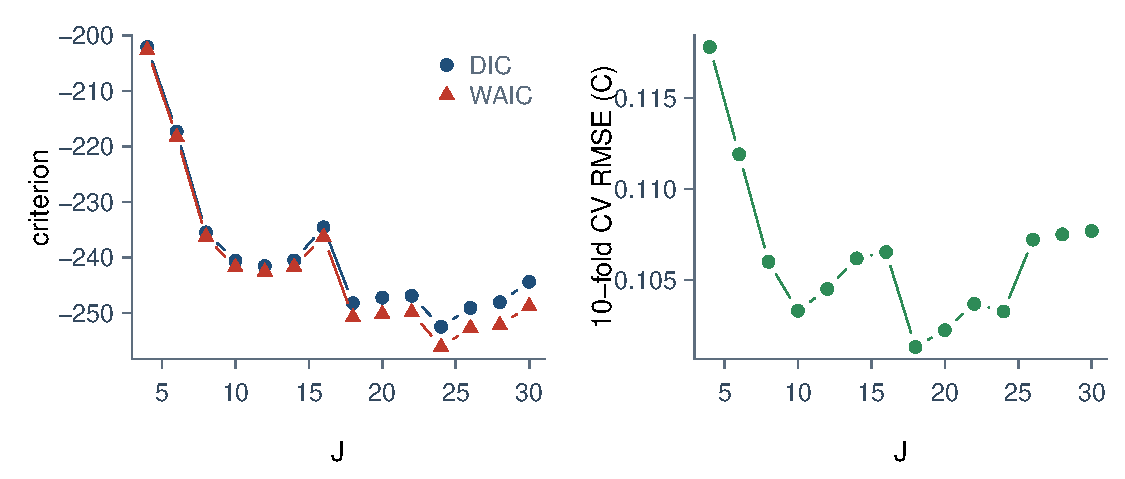
\includegraphics[width=0.98\linewidth]{ex12_selection.pdf}\end{center}
DIC and WAIC are minimised at $J=24$; 10-fold CV at $J=18$. All three criteria are nearly flat for $J$ between about 10 and 24 (CV RMSE varies by only $0.002^\circ$C), so any $J$ in that range is defensible; the zig-zag is partly Monte Carlo and fold-to-fold noise.

\step{(c) PPCs for $J=24$.}
\begin{center}
\begin{tabular}{lcccc}\toprule
 & lag-1 ACF of residuals & kurtosis & max $|\varepsilon|$ & sign changes\\\midrule
observed & 0.235 & $-0.53$ & 0.223 & 61.6\\
replicated & $-0.007$ & $-0.08$ & 0.255 & 70.5\\
PPP & \textbf{0.005} & 0.87 & 0.77 & 0.91\\\bottomrule
\end{tabular}
\end{center}
The residuals are positively autocorrelated (warm years follow warm years beyond the smooth trend; e.g.\ El Ni\~no episodes) and change sign less often than independent noise would. Marginal shape (kurtosis, extremes) is fine.

\begin{answer}
(a) DIC and WAIC choose $J=24$. (b) 10-fold CV chooses $J=18$; the criteria are flat for $J\approx10$--24. (c) The selected fit fails the residual-autocorrelation check (PPP 0.005): add AR(1) errors (or a smoother with a penalty) for honest uncertainty; the curve itself is fine.
\end{answer}

\begin{takeaway}
When criteria are flat over a range, report that range --- and remember that autocorrelated errors make DIC/WAIC/CV favour overly wiggly curves.
\end{takeaway}

% ================================================================= Exercise 13
\exercise{6.13 --- $t$ vs.\ Gaussian for the galaxies: posterior predictive checks}

\begin{problem}{13}
Open and plot the galaxies data in R using the code below,
\begin{lstlisting}
> library(MASS)
> data(galaxies)
> ?galaxies
> Y <- galaxies
> n <- length(Y)
> hist(Y,breaks=25)
\end{lstlisting}
Model the observations $Y_1,\dots,Y_{82}$ using the Student's t-distribution with location $\mu$, scale $\sigma$ and degrees of freedom $k$. Assume prior distributions $\mu\sim\dist{Normal}(0,10000^2)$, $1/\sigma^2=\tau\sim\dist{Gamma}(0.01,0.01)$ and $k\sim\dist{Uniform}(1,30)$.
\begin{enumerate}[(a)]
\item Use posterior predictive checks to evaluate whether the t distribution captures the mean, variance, skewness and kurtosis of the data.
\item Repeat this analysis with a Gaussian model.
\end{enumerate}
\end{problem}

\begin{restate}
Fit a $t$ and a normal distribution to the galaxy velocities and check whether replicated data match the observed mean, variance, skewness and kurtosis.
\end{restate}

\begin{recall}
Student-$t$ Gibbs sampler (Exercise 3.9). Sample skewness $\frac{\frac1n\sum(Y_i-\bar Y)^3}{s^3}$ and excess kurtosis $\frac{\frac1n\sum(Y_i-\bar Y)^4}{s^4}-3$ (both 0 for a normal distribution).
\end{recall}

\begin{keyidea}
A PPC passes when the observed statistic is a typical value of the replicated statistic (PPP not close to 0 or 1).
\end{keyidea}

\solution
\step{Fits.} $t$ model: posterior as in Exercise 3.9 ($\mu\approx21{,}100$, $\sigma\approx2{,}240$, $k\approx2.1$). Gaussian model (same priors for $\mu,\tau$): $\mu=20{,}776$ (19{,}764--21{,}781), $\sigma=4{,}603$ (3{,}952--5{,}395).
\step{Checks} (5{,}000 replicated datasets of 82 values each):
\begin{center}
\small
\begin{tabular}{l|c|cc|cc}\toprule
 & & \multicolumn{2}{c|}{$t$ model} & \multicolumn{2}{c}{Gaussian model}\\
Statistic & observed & 95\% replicated interval & PPP & 95\% replicated interval & PPP\\\midrule
mean & 20{,}828 & (18{,}870, 23{,}280) & 0.65 & (19{,}310, 22{,}210) & 0.47\\
variance & $2.08\times10^7$ & $(0.8\times10^7,\ 67\times10^7)$ & 0.58 & $(1.3\times10^7,\ 3.2\times10^7)$ & 0.49\\
skewness & $-0.43$ & $(-6.9,\ 6.7)$ & 0.59 & $(-0.51,\ 0.49)$ & 0.95\\
kurtosis & 2.14 & (0.46, 64.9) & 0.85 & $(-0.85,\ 1.02)$ & \textbf{0.002}\\\bottomrule
\end{tabular}
\end{center}
\begin{center}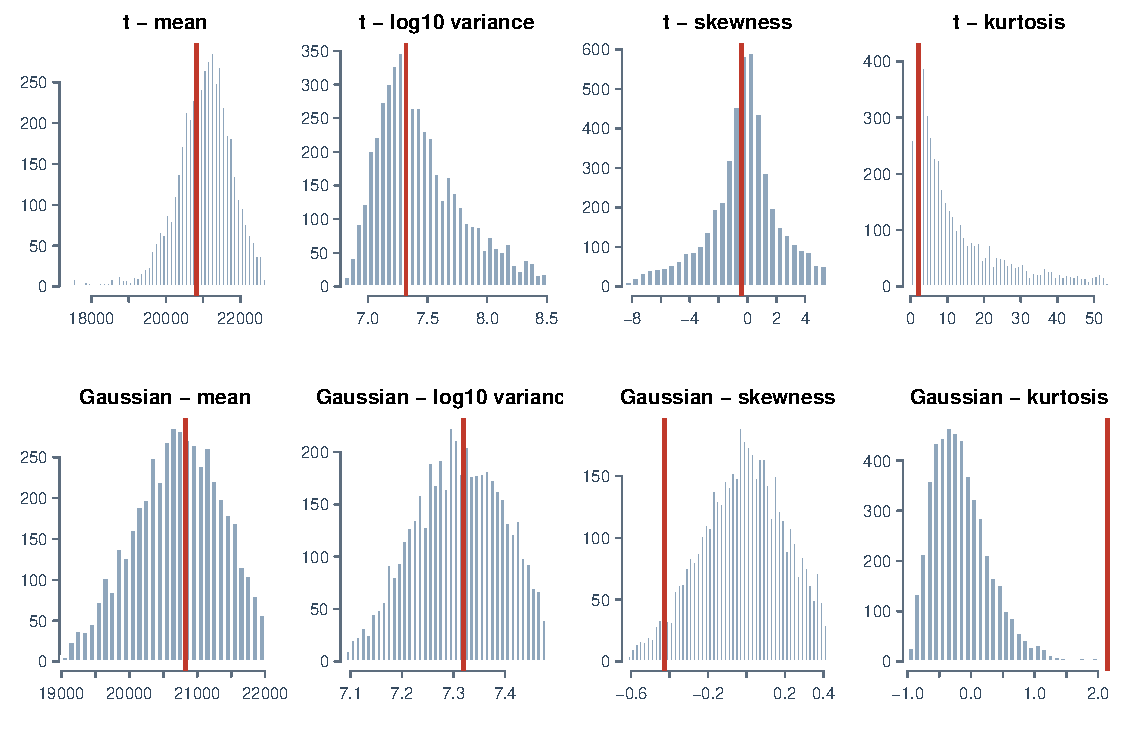
\includegraphics[width=0.98\linewidth]{ex13_ppc.pdf}\end{center}

\begin{answer}
(a) The $t$ model passes all four checks (PPP 0.58--0.85) --- but only because with $k\approx2$ its replicated variance, skewness and kurtosis are so variable that almost anything is ``typical''. (b) The Gaussian model matches the mean and variance but fails kurtosis badly (PPP 0.002: the data have far heavier tails than a normal), and skewness is borderline (PPP 0.95).
\end{answer}

\begin{takeaway}
Passing PPCs is not proof of a good model: the $t$ ``passes'' by being vague, yet Exercises 3.9 and 4.13 showed it misses the multi-modality. Add statistics that target the suspected failure (e.g.\ the number of modes or the gap between clusters).
\end{takeaway}

% ================================================================= Exercise 14
\exercise{6.14 --- Strengths and weaknesses of model-selection tools}

\begin{problem}{14}
For each model selection approach below, give an advantage and a limitation of the approach and a hypothetical situation where it would be a good option.
\begin{enumerate}[(a)]
\item Bayes factors
\item Stochastic search variable selection
\item Cross validation
\item DIC/WAIC
\end{enumerate}
\end{problem}

\begin{restate}
Compare four model-selection tools: what each does well, what it does badly, and when to use it.
\end{restate}

\begin{keyidea}
Bayes factors and SSVS ask ``which model is \emph{true}?'' (prior predictive); CV and DIC/WAIC ask ``which model \emph{predicts} best?'' (posterior predictive).
\end{keyidea}

\solution
\begin{center}
\small
\renewcommand{\arraystretch}{1.35}
\begin{tabular}{p{0.13\linewidth}p{0.25\linewidth}p{0.25\linewidth}p{0.27\linewidth}}\toprule
Approach & Advantage & Limitation & Good situation\\\midrule
(a) Bayes factors & Coherent: gives posterior model probabilities and can support the null; automatically penalises complexity. & Very sensitive to vague priors (Lindley's paradox, Exercise 5.3); marginal likelihoods can be hard to compute. & Comparing a few scientifically motivated models with informative priors, e.g.\ ``does a drug have an effect?'' with a prior based on earlier trials.\\
(b) SSVS & Explores huge model spaces ($2^p$) and gives inclusion probabilities and model-averaged predictions. & Inherits BF prior sensitivity; mixes poorly and dilutes probabilities with collinear predictors (Exercise 4). & Choosing among $p=10$--100 candidate predictors, e.g.\ which neighbourhood variables affect house prices (Exercise 5.9).\\
(c) Cross validation & Directly measures out-of-sample prediction; few assumptions; works for any model, even non-Bayesian ones. & Computationally expensive (refit $K$ times); noisy for small $n$; needs care with dependent data (time series, clusters). & Choosing a predictive model, e.g.\ which covariates best forecast ozone (Exercise 1).\\
(d) DIC / WAIC & Cheap (one MCMC run); estimate predictive accuracy and effective model size. & Approximations; DIC can misbehave (negative $p_D$, multimodal posteriors); both assume roughly independent observations. & Quickly comparing several fitted hierarchical models, e.g.\ random-effect distributions for the Gambia data (Section 6.4).\\\bottomrule
\end{tabular}
\end{center}

\begin{answer}
See the table: Bayes factors --- coherent but prior-sensitive (use with informative priors); SSVS --- searches many models but struggles with collinearity (use for moderate $p$ variable selection); CV --- assumption-light prediction measure but costly (use for predictive model choice); DIC/WAIC --- cheap predictive approximations (use to compare hierarchical models fitted by MCMC).
\end{answer}

\begin{takeaway}
Decide first whether the goal is \emph{explanation} (which model is true?) or \emph{prediction} (which model predicts best?) --- that decides the tool.
\end{takeaway}

\end{document}
